\documentclass[border=10pt]{standalone}

\usepackage{tikz}
\usepackage{tikzsymbols}
\usetikzlibrary{calc,patterns,shapes.geometric}

\def\centerarc[#1](#2)(#3:#4:#5){\draw[#1] ($(#2)+({#5*cos(#3)},{#5*sin(#3)})$) arc (#3:#4:#5);}

\begin{document}
	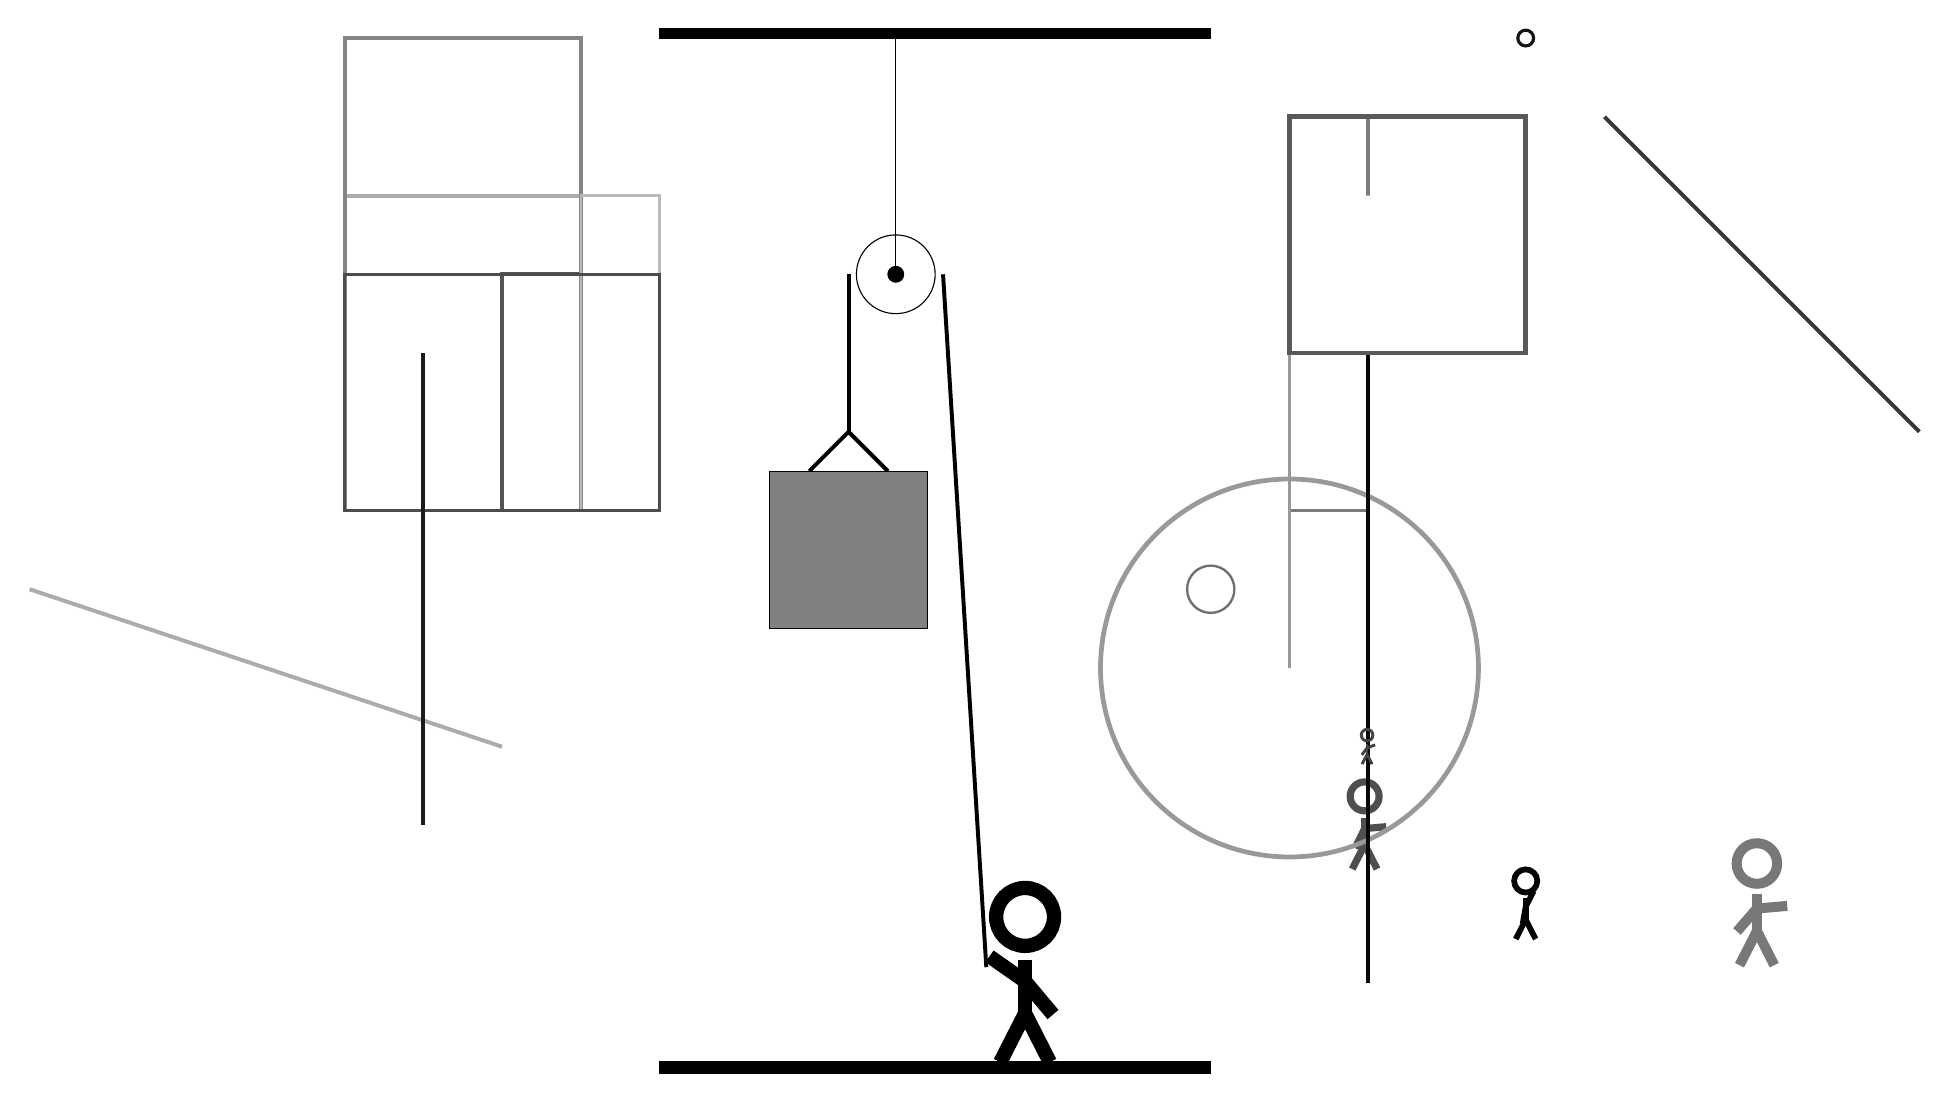
\begin{tikzpicture}
		%%%%% START %%%%%
		
		\draw[fill=black] (-2, 10) rectangle (5, 10.125);
		
		\draw (1, 7) circle (0.5);
		\draw[fill=black] (1, 7) circle (0.1);
		\draw (1, 10) -- (1, 7);
		
		\draw[line width=0.5mm] (-0.1, 4.5) -- (0.4, 5.0) -- (0.9, 4.5);
		\draw[fill=black!50] (-0.6, 4.5) rectangle (1.4, 2.5);
		
		\draw[line width=0.5mm, color=black!67] (-3, 4) rectangle (-4, 7);
		
		\draw[line width=0.3mm, color=black!52] (7, 4) rectangle (6, 6);
		\node[line width=0.2mm, color=black!69] at (7, 0) {\Strichmaxerl[5][64][5]};
		\draw [line width=0.3mm, color=black!56](5, 3) circle (0.3);
		\draw[line width=0.5mm, color=black!79](10, 9) -- (14, 5);
		\draw[line width=0.5mm, color=black!33](-4, 1) -- (-10, 3);
		
		\draw[line width=0.5mm, color=black!51] (7, 9) rectangle (7, 8);
		\draw [line width=0.6mm, color=black!40](6, 2) circle (2.4);
		\node[line width=0.4mm, color=black!99] at (9, -1) {\Strichmaxerl[4][80][63]};
		\draw[line width=0.5mm, color=black!32] (-3, 10) rectangle (-6, 8);
		\draw[line width=0.5mm, color=black!48] (-3, 10) rectangle (-6, 4);
		\draw[line width=0.3mm, color=black!27] (-3, 4) rectangle (-2, 8);
		\draw[line width=0.5mm, color=black!40](6, 2) -- (6, 8);
		\draw[line width=0.4mm, color=black!70] (-2, 4) rectangle (-6, 7);
		\draw[line width=0.5mm, color=black!97] (7, 6) rectangle (7, -2);
		\draw [line width=0.4mm, color=black!40](9, 2) circle (0.0);
		\draw[line width=0.5mm, color=black!89](-5, 6) -- (-5, 0);
		\draw[line width=0.6mm, color=black!65] (6, 9) rectangle (9, 6);
		\node[line width=0.3mm, color=black!53] at (12, -1) {\Strichmaxerl[7][49][5]};
		\draw [line width=0.4mm, color=black!92](9, 10) circle (0.1);
		\node[line width=0.3mm, color=black!74] at (7, 1) {\Strichmaxerl[2][53][21]};
		
		
		\draw[line width=0.5mm] (0.4, 7) -- (0.4, 5.0);
		\centerarc[line width=0.5mm](1, 7)(0:180:0.6);
		\draw[line width=0.5mm](1.6, 7) -- (2.15, -1.8);
		
		\node at (2.6, -1.9) {\Strichmaxerl[10][-35][-50]};
		
		\draw[fill=black] (-2, -3) rectangle (5, -3.15);
		
		%%%%% END %%%%%
	\end{tikzpicture}
\end{document}